\chapter{Les étapes d'une approche data-driven}
\chapterintrobox{Une approche de pronostic \acrlong{dd} (une approche qui s’appuie sur des données opérationnelles historiques pour construire un modèle qui est utilisé pour prédire la durée de vie utile restante) doit passer par de multiples étapes—de l’acquisition de données jusqu’à l’estimation de la durée de vie utile restante. Dans ce chapitre, ces différentes étapes seront examinées en détail.}

\section{Aquisition de données}
Un signal est une fonction qui transmet des informations sur le comportement d'un système ou les attributs d'un phénomène. les signaux se produisent naturellement et sont également synthétisés. Un signal n'est pas nécessairement une grandeur électrique. Cependant, pour effectuer des activités telles que la synthèse, le transport, l'enregistrement, l'analyse et la modification de signaux, il est souvent pratique d'utiliser un signal sous la forme d'une grandeur électrique \cite{Priemer1990}.

L'acquisition de données est un processus de capture et de stockage de différents types de données de surveillance (signaux) provenant de divers capteurs installés sur l'équipement surveillé. C'est le premier processus de pronostic des machines, qui fournit des informations de base de surveillance d'état (\acrlong{cm}) pour les processus suivants. Un système d'acquisition de données est composé de capteurs, de dispositifs de transmission de données et de dispositifs de stockage de données \cite{Lei2018}. Les données de surveillance d'état sont très versatiles. Il peut s'agir de données sur les vibrations, de données acoustiques, de données d'analyse d'huile, de données sur la température, la pression, l'humidité, les conditions météorologiques ou l'environnement, etc. Les différents capteurs, tels que les micro-capteurs, les capteurs à ultrasons et les capteurs d'émission acoustique ont été conçus pour collecter différents types de données. Les technologies sans fil, telles que Bluetooth, ont fourni une solution alternative à la communication de données à un prix avantageux \cite{Jardine2006}.

Bien que la recherche sur des concepts avancés comme les réseaux de capteurs sans fil et la récolte d’énergie pour alimenter des capteurs autonomes soit en cours, l’acquisition de données (capteurs) et la manipulation sont aujourd’hui plutôt bien établies. Par conséquent, une grande partie de la recherche dans cette discipline se concentre sur l’analyse des données obtenues pour en extraire de l’information \cite{Tinga2014}. Parce que cette discipline est bien développée, beaucoup de nouvelles installations et techniques d’acquisition de données ont été conçues et appliquées dans les industries modernes. Ces installations puissantes et polyvalentes ont rendu l’acquisition de données pour la mise en œuvre du PHM plus pratique et plus faisable \cite{Lei2016}.

\section{Extraction de Caractéristiques}
L'approche de pronostic data-driven est principalement utilisée lorsqu'il est difficile de comprendre le comportement physique d'un système complexe. La compréhension du comportement et de l'interaction des différents éléments qui conduisent à la dégradation des machines est le point de départ pour développer un modèle physique pour les pronostics.
D'autre part, cette approche utilise des données de surveillance des conditions pour modéliser implicitement son comportement. Les modèles utilisés dans l'approche data-driven utilisent des données de surveillance pour modéliser un comportement complexe et capturer des modèles complexes, mais ils sont considérés comme des boîtes noires : ils ne fournissent pas nécessairement un aperçu du processus.
En général, la performance de ces modèles dépend de la qualité des données d'entrée (données). La partie humaine ne peut pas effectuer la tâche que le modèle effectue, mais le traitement des données d'entrée peut augmenter considérablement les résultats. Ce traitement est nécessaire parce que les données des capteurs sur lesquelles le modèle repose sont généralement redondantes, bruyantes et incomplètes, ces imperfections sont dues à de nombreuses raisons.


\subsection{Traitement du signal}
Le traitement du signal est l'étude et l'analyse des signaux stockés afin de révéler leurs propriétés—qui peuvent ne pas être apparentes au premier abord, en utilisant un ensemble d'algorithmes et de techniques. Dans le contexte de la surveillance de l'état, ces propriétés révélées par le traitement du signal peuvent être révélatrices de santé de la machine.
Le traitement du signal est un sous-domaine bien établi et mature du génie électrique, avec de nombreuses techniques et algorithmes proposés dans la littérature.


Le traitement du signal peut être classé en trois catégories : \textbf{Analyse Temporelle}, \textbf{Analyse Fréquentielle} et \textbf{Analyse Temps–Fréquence}.

\subsubsection{Analyse Temporelle}
Les mesures originales des signaux qui sont généralement échantillonnés de manière répétée entre des intervalles de temps prédéfinis sont sous forme de domaine temporel. Ainsi, l'analyse du domaine temporel est directement basée sur la mesure originale \cite{Lei2016}.


\subsubsection{Analyse Fréquentielle}
L'analyse du domaine fréquentiel est basée sur les signaux transformés dans le domaine fréquentiel. L'avantage de l'analyse en domaine fréquentiel par rapport à l'analyse en domaine temporel est sa capacité à décomposer les signaux originaux en une série de composantes fréquentielles. L'analyse du domaine fréquentiel la plus utilisée est l'analyse du spectre au moyen de la transformée de Fourier rapide (FFT). L'idée principale de l'analyse spectrale est d'isoler et de localiser certaines composantes de fréquence d'intérêt relatives aux caractéristiques de défaut des machines \cite{Lei2016a}.


\subsubsection{Analyse Temps–Fréquence}
Le problème de l'analyse du domaine temporel et de l'analyse du domaine fréquentiel est que chacune d'elles ne dispose d'aucune information sur l'autre domaine (l'analyse du domaine temporel ne dispose d'aucune information sur le domaine fréquentiel, et l'analyse du domaine fréquentiel ne dispose d'aucune information sur la position dans le temps).

Ainsi, l'analyse du domaine temps-fréquence, qui
étudie les signaux de mesure dans les domaines du temps et des fréquences, a été appliquée à l'analyse des signaux de mesure non stationnaires. L'analyse temps-fréquence décrit les caractéristiques des signaux de mesure dans les fonctions bidimensionnelles du temps et de la fréquence afin de mieux révéler les modes de défaillance des machines.


La figure \ref{fig:signal-processing} présente les différentes techniques utilisées pour chaque type d'analyse:

\begin{figure}[h]
    \centering
	\documentclass[12pt]{article}

\usepackage{tikz}
\usetikzlibrary{positioning,arrows}

\begin{document}
	
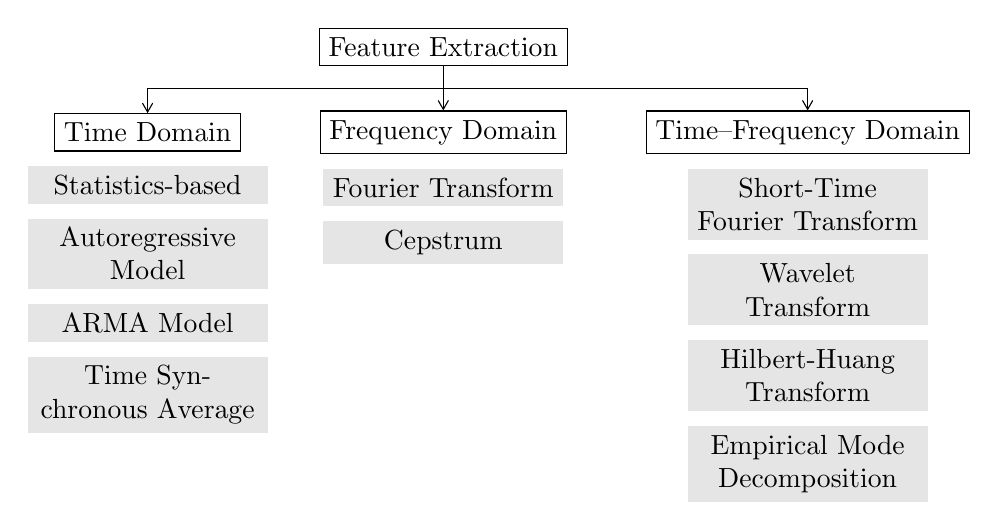
\begin{tikzpicture}
\tikzstyle{element}=[draw,rectangle]
\tikzstyle{entity}=[fill=gray!20,align=center, text width=8em]
\node[element] (fe) {Feature Extraction};


\node[element,below = 1.6em of fe] (fd) {Frequency Domain};
\node[element,left = of fd] (td) {Time Domain};
\node[element,right = of fd] (tfd) {Time--Frequency Domain};

\node[entity,below =.5em of td] (stat) {Statistics-based};
\node[entity,below =.5em of stat] (arm) {Autoregressive Model};
\node[entity,below =.5em of arm] (arma) {ARMA Model};
\node[entity,below =.5em of arma] (tsa) {Time Synchronous Average};

\node[entity,below =.5em of fd] (fft) {Fourier Transform};
\node[entity,below =.5em of fft] (cep) {Cepstrum};

\node[entity,below =.5em of tfd] (stft) {Short-Time Fourier Transform};
\node[entity,below =.5em of stft] (wt) {Wavelet Transform};
\node[entity,below =.5em of wt] (hht) {Hilbert-Huang Transform};
\node[entity,below =.5em of hht,align=center, text width=8em] (emd) {Empirical Mode Decomposition};

\draw[->,>=angle 60] (fe.south) -- ++(0,0) -- ++(0,-.8em) -| (td);
\draw[->,>=angle 60] (fe.south) -| (fd);
\draw[->,>=angle 60] (fe.south) -- ++(0,0) -- ++(0,-.8em) -| (tfd);
\end{tikzpicture}


\end{document}
    \caption{Techniques de traitement du signal dans les différents domaines}
    \label{fig:signal-processing}
\end{figure}

\subsection{Reduction de la dimensionalité}
La réduction de la dimensionnalité se réfère au processus consistant à prendre des données à haute dimension et à trouver une bonne représentation de ces données dans une dimension inférieure tout en préservant ses caractéristiques originales. La réduction de la dimensionnalité est effectuée pour l'extraction de caractéristiques en trouvant les principales composantes ou pour la visualisation (en réduisant le nombre de dimensions à 2 ou 3).
Il existe de nombreuses techniques et algorithmes de réduction de la dimensionnalité comme:
\begin{itemize}
    \item Principal Component Analysis (PCA)
    \item Autoencoders
    \item t-Distributed Stochastic Neighbor Embedding (t-SNE)
\end{itemize}

Il faut noter que pour les pronostics, où les données utilisées consistent en des entrées de capteurs où chaque variable a une signification physique et une interprétation directe, le fait d'effectuer une réduction de la dimensionnalité donnera les principales composantes, mais les nouvelles variables \textit{perdront leur interprétabilité physique} et \textit{devront être traitées comme des abstractions}.


\section{Diagnostic}
Le diagnostic se résume à un processus d'identification et de détermination de la relation entre les informations obtenues dans l'espace de mesure et les modes de défaillance des machines dans l'espace de défaillance. Le diagnostic comporte trois grandes étapes, à savoir la détection des défauts, l'isolation des défauts et l'identification des défauts. La détection des défauts est une tâche qui consiste à indiquer si un défaut a s'est déjà produite dans les machines surveillées. L'isolation des défauts consiste à trouver la composante de la défaillance et la position de la défaillance. L'identification des défauts est la dernière étape du diagnostic, qui tente de déterminer le mode et la gravité de la défaillance. Les trois étapes sont en corrélation entre eux. Cette dernière étape repose sur les résultats de la première et ne peut donc pas être réalisée individuellement \cite{Lei2016b}.
\section{Pronostic}

Le diagnostic est l'analyse de l'événement postérieur et le pronostic est l'analyse de l'événement antérieur. Le pronostic est beaucoup plus efficace que le diagnostic pour obtenir des performances sans arrêt de production. Le diagnostic est toutefois nécessaire lorsque la prédiction des erreurs de pronostic échoue et qu'une erreur se produit \cite{Jardine2006}.
\section{Décision de la maintenance}
\section{Conclusion}
